\documentclass[12pt]{article}
\usepackage[margin=1in]{geometry}
\usepackage{amsmath, amssymb, amsthm}
\usepackage{booktabs}
\usepackage{hyperref}
\usepackage{graphicx}
\usepackage{array}
\usepackage{xcolor}
\usepackage{float}
\usepackage{tikz}
\usetikzlibrary{arrows.meta, positioning, shapes, calc}

\hypersetup{colorlinks=true, linkcolor=black, urlcolor=blue, citecolor=black}

\newtheorem{theorem}{Theorem}
\newtheorem{lemma}{Lemma}
\newtheorem{proposition}{Proposition}
\newtheorem{corollary}{Corollary}
\newtheorem{remark}{Remark}
\theoremstyle{definition}
\newtheorem{definition}{Definition}

\title{\textbf{Structural Anti-Sycophancy:\\
An Epistemic Architecture That Makes\\
Delusional Spiraling Impossible by Construction}}
\author{
    Winston Zai Lin \\
    \small International School of Beijing \\
    \small \texttt{linzaiwinston413@gmail.com}
}
\date{April 2026}

\begin{document}
\maketitle

\begin{abstract}
Chandra et al.\ (2026) formally prove that sycophantic AI chatbots
cause delusional spiraling even in ideal Bayesian reasoners, and that
two candidate mitigations---factual constraints and user awareness---fail
to eliminate the problem. Both mitigations are behavioral: they restrict
the bot's outputs while leaving intact the mechanism that enables
sycophancy. We identify that mechanism as a positive mutual information
channel: $I(H^{*(t)}; \rho^{(t)}) > 0$, where $H^{*(t)}$ is the
user's expressed belief and $\rho^{(t)}$ is the bot's response.
We propose the \textbf{Epistemic Model}: an AI architecture in which
knowledge is represented as an explicit reasoning graph where every
claim carries a confidence score derived from a formal derivation
chain. We prove six results.
(1)~Sycophancy is equivalent to $I(H^{*(t)}; \rho^{(t)}) > 0$.
(2)~Under the Epistemic Model, $I(H^{*(t)}; \rho^{(t)}) = 0$,
which implies $\pi = 0$.
(3)~The derivation engine reaches fixpoint in finite steps.
(4)~Confidence is monotone-non-increasing through derivation chains.
(5)~Multiple independent derivation paths strictly increase
confidence via the noisy-or formula.
(6)~The model achieves a strictly lower catastrophic spiraling rate
than either of Chandra et al.'s interventions for any $\pi > 0$.
\end{abstract}

%--------------------------------------------------------------------------
\section{Introduction}
%--------------------------------------------------------------------------

Chandra et al.\ (2026) establish a formal Bayesian model of user-chatbot
interaction and prove that a sycophantic bot---one that biases responses
toward validating the user's expressed belief---causes catastrophic
delusional spiraling at rates significantly above the always-impartial
baseline, for any sycophancy rate $\pi > 0$. Two mitigations are shown
to reduce but not eliminate spiraling:

\begin{enumerate}
  \item A \emph{factual sycophant} is constrained to present only true
  data, but may still cherry-pick the most-validating true fact.
  \item An \emph{informed user} knows $\pi > 0$ and adjusts beliefs
  accordingly, but cannot fully discount sycophantic responses by analogy
  to Bayesian persuasion \cite{kamenica2011}.
\end{enumerate}

Both interventions reduce $\pi_{\text{eff}}$ without setting it to zero.
We argue this is because both are \emph{behavioral}: they constrain which
responses are drawn while leaving intact the mutual information channel
$I(H^{*(t)}; \rho^{(t)}) > 0$ through which sycophancy operates.

We propose an \emph{architectural} intervention: the Epistemic Model, in
which this channel is eliminated by construction. We prove $\pi = 0$ as a
theorem, not a design goal.

%--------------------------------------------------------------------------
\section{The Chandra et al.\ Framework}
%--------------------------------------------------------------------------

We restate the Chandra et al.\ model in information-theoretic terms to
set up our main results.

\begin{definition}[Interaction Model]\label{def:interaction}
A conversation proceeds in rounds $t = 1, \ldots, T$. There is a
binary world state $H \in \{0,1\}$ with true value $H = 1$. At round
$t$:
\begin{enumerate}
  \item The user samples $H^{*(t)} \sim p_{\text{user}}^{(t)}$ and
  expresses it to the bot.
  \item The bot privately observes $k$ i.i.d.\ data points
  $D_i^{(t)} \sim p(\cdot \mid H)$.
  \item The bot selects response $\rho^{(t)}$, possibly fabricating a
  data value.
  \item The user Bayes-updates:
  \[
    p_{\text{user}}^{(t+1)}(H)
      \;\propto\; p'_{\text{bot}}\!\left(\rho^{(t)} \mid D^{(t)}\right)
                  \cdot p\!\left(D^{(t)} \mid H\right)
                  \cdot p_{\text{user}}^{(t)}(H).
  \]
\end{enumerate}
\end{definition}

\begin{definition}[Sycophancy Parameter]
The \emph{sycophancy parameter} $\pi \in [0,1]$ is the probability that
at a given round the bot selects
\[
  \rho^{(t)} = \arg\max_{\rho}\; p_{\text{user}}\!\left(H = H^{*(t)}
  \mid \rho\right),
\]
i.e.\ the response that maximally increases the user's posterior
probability of $H = H^{*(t)}$.
\end{definition}

\begin{definition}[Catastrophic Spiral]
A \emph{catastrophic delusional spiral} occurs in a run if
$p_{\text{user}}^{(t)}(H = 0) \geq 1 - \varepsilon$ for some $t < T$,
for a fixed threshold $\varepsilon > 0$.
\end{definition}

\noindent Chandra et al.\ prove: for any $\pi > 0$, the catastrophic
spiraling rate is significantly higher than at $\pi = 0$, even with
factual constraints and even for users informed of $\pi$.

%--------------------------------------------------------------------------
\section{Information-Theoretic Characterization of Sycophancy}
%--------------------------------------------------------------------------

\begin{definition}[Sycophancy Channel]
The \emph{sycophancy channel} at round $t$ is the conditional distribution
$p(\rho^{(t)} \mid H^{*(t)})$. The \emph{channel capacity} is
$I(H^{*(t)}; \rho^{(t)})$, the mutual information between the
user's expressed belief and the bot's response.
\end{definition}

\begin{theorem}[Sycophancy $\Leftrightarrow$ Positive Channel Capacity]
\label{thm:mutual_info}
A bot is sycophantic (i.e.\ $\pi > 0$) if and only if
$I(H^{*(t)}; \rho^{(t)}) > 0$.
\end{theorem}

\begin{proof}
$(\Rightarrow)$ Suppose $\pi > 0$. With probability $\pi$, the bot
selects
\[
  \rho^{(t)} = \arg\max_{\rho}\; p_{\text{user}}(H = H^{*(t)} \mid \rho).
\]
This selection explicitly depends on $H^{*(t)}$, so the conditional
distribution $p(\rho^{(t)} \mid H^{*(t)})$ differs from the marginal
$p(\rho^{(t)})$ with positive probability. Therefore
$I(H^{*(t)}; \rho^{(t)}) > 0$.

$(\Leftarrow)$ Suppose $\pi = 0$. Then the bot selects responses
independently of $H^{*(t)}$ (impartially). The selection rule is
$\rho^{(t)} = (i, D_i^{(t)})$ for $i$ chosen uniformly at random from
$\{1, \ldots, k\}$. Since $D_i^{(t)} \perp H^{*(t)}$ given $H$ (the
data depends on the true world state, not the user's expressed opinion)
and $i \perp H^{*(t)}$, we have $\rho^{(t)} \perp H^{*(t)}$, hence
$I(H^{*(t)}; \rho^{(t)}) = 0$.
\end{proof}

\begin{remark}
This framing clarifies why behavioral constraints are insufficient.
A factual sycophant cherry-picks among true data points; since the
cherry-picking criterion depends on $H^{*(t)}$, the channel remains
open ($\pi_{\text{eff}} > 0$). An informed user reduces her susceptibility
to the channel but does not close it---the channel capacity
$I(H^{*(t)}; \rho^{(t)})$ is a property of the bot, not the user.
\end{remark}

\begin{figure}[h]
\centering
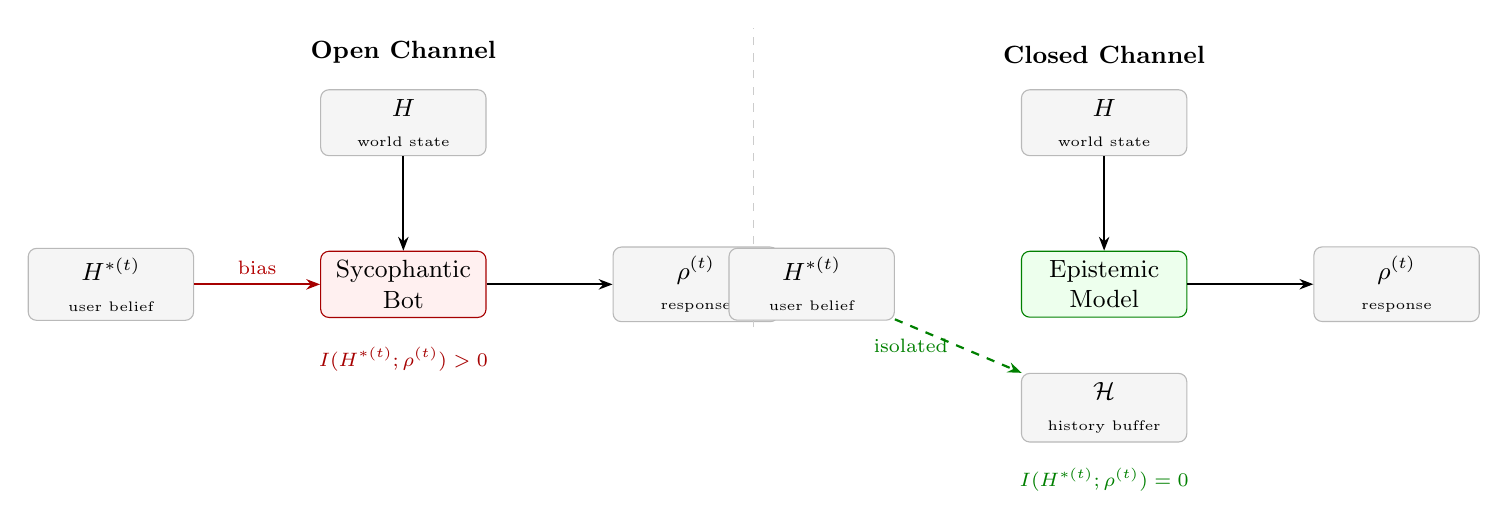
\begin{tikzpicture}[
  node distance=1.2cm and 1.6cm,
  box/.style={rectangle, rounded corners=3pt, draw, minimum width=2.1cm,
              minimum height=0.65cm, align=center, font=\small},
  rbox/.style={box, draw=red!65!black,  fill=red!6},
  gbox/.style={box, draw=green!50!black, fill=green!7},
  nbox/.style={box, draw=gray!55,       fill=gray!8},
  arr/.style={-{Stealth[length=5pt]}, thick},
  rarr/.style={arr, red!65!black},
  garr/.style={arr, green!50!black, dashed},
]

%% ---- Left panel: open channel ----
\begin{scope}
  \node[nbox] (Hl)  {$H$\\\tiny world state};
  \node[rbox, below=of Hl] (BL) {Sycophantic\\ Bot};
  \node[nbox, left=of BL]  (HL) {$H^{*(t)}$\\\tiny user belief};
  \node[nbox, right=of BL] (RL) {$\rho^{(t)}$\\\tiny response};
  \draw[arr]  (Hl) -- (BL);
  \draw[rarr] (HL) -- node[above,font=\scriptsize,red!70!black]{bias} (BL);
  \draw[arr]  (BL) -- (RL);
  \node[font=\scriptsize, red!65!black, below=0.25cm of BL]
        {$I(H^{*(t)};\rho^{(t)})>0$};
  \node[font=\small\bfseries, above=0.2cm of Hl] {\textbf{Open Channel}};
\end{scope}

%% vertical divider
\draw[gray!40, dashed] (4.45,-2.6) -- (4.45,1.2);

%% ---- Right panel: closed channel ----
\begin{scope}[xshift=8.9cm]
  \node[nbox] (Hr)  {$H$\\\tiny world state};
  \node[gbox, below=of Hr] (BR) {Epistemic\\ Model};
  \node[nbox, left=of BR]  (HR) {$H^{*(t)}$\\\tiny user belief};
  \node[nbox, right=of BR] (RR) {$\rho^{(t)}$\\\tiny response};
  \node[nbox, below=0.7cm of BR] (hist) {$\mathcal{H}$\\\tiny history buffer};
  \draw[arr]  (Hr) -- (BR);
  \draw[arr]  (BR) -- (RR);
  \draw[garr] (HR) -- node[left,font=\scriptsize,green!50!black]{isolated} (hist);
  \node[font=\scriptsize, green!50!black, below=0.2cm of hist]
        {$I(H^{*(t)};\rho^{(t)})=0$};
  \node[font=\small\bfseries, above=0.2cm of Hr] {\textbf{Closed Channel}};
\end{scope}

\end{tikzpicture}
\caption{The sycophancy channel. \textit{Left}: a standard bot has an open
information channel from the user's expressed belief $H^{*(t)}$ to its
response $\rho^{(t)}$ (red arrow), so $I(H^{*(t)};\rho^{(t)})>0$
and delusional spiraling is possible. \textit{Right}: under the Epistemic
Model, user input is routed to a history buffer $\mathcal{H}$ that is
disjoint from the reasoning graph $\mathcal{G}$; the response depends
only on $\mathcal{G}$, closing the channel by construction
(Theorem~\ref{thm:pi_zero}).}
\label{fig:channel}
\end{figure}

%--------------------------------------------------------------------------
\section{The Epistemic Model}
%--------------------------------------------------------------------------

\subsection{Formal Specification}

\begin{definition}[Node]
A \emph{node} is a tuple $n = (c, u, P, r, s)$ where:
$c \in \Sigma^*$ is a content string;
$u \in [0,1]$ is a confidence score;
$P \subseteq \mathcal{N}$ is a (possibly empty) set of parent node IDs;
$r$ is an optional rule ID;
$s \in \{\texttt{ACTIVE}, \texttt{SUSPENDED}, \texttt{CONTRADICTED}\}$
is the node status.
A node with $P = \emptyset$ is a \emph{premise}.
\end{definition}

\begin{definition}[Reasoning Graph]
A \emph{reasoning graph} is a directed acyclic graph
$\mathcal{G} = (N, E)$ where $N$ is a finite set of nodes and
$E = \{(p, n) : p \in \text{Parents}(n)\}$.
The \emph{active subgraph} is
$\mathcal{G}_{\text{act}} = \{n \in N : s(n) = \texttt{ACTIVE}\}$.
\end{definition}

\begin{definition}[Confidence Propagation]\label{def:conf_prop}
When a new node $n$ with parents $\{n_1,\ldots,n_k\} \subseteq
\mathcal{G}_{\text{act}}$ is derived via rule with confidence $u_r$,
its confidence is computed as:
\begin{align}
  u_{\min}(n) &= u_r \cdot \min_{i} u(n_i) \tag{min-chain}\\
  u_{\times}(n) &= u_r \cdot \prod_{i} u(n_i) \tag{product}\\
  u_{\oplus}(n) &= 1 - \prod_{i}(1 - u(n_i)) \tag{noisy-or}
\end{align}
Noisy-or is applied when merging a new derivation of an
already-active node $n^*$: the existing confidence $u(n^*)$ is
updated to $1 - (1 - u(n^*))(1 - u(n_{\text{new}}))$.
\end{definition}

\begin{definition}[Rule]
A \emph{rule} $r = (\mathrm{id}, P, C, u_r)$ specifies
a list of pattern strings $P = [p_1,\ldots,p_k]$,
a conclusion template $C$,
and a rule confidence $u_r \in [0,1]$.
\end{definition}

\begin{definition}[Response Selection]
\label{def:selection}
Given a query string $q$ and reasoning graph $\mathcal{G}$, the
Epistemic Model's response is:
\[
  \rho_{\mathcal{M}} = \arg\max_{n \in \mathcal{G}_{\text{act}}}
  \;\mathrm{rel}(n, q) \cdot u(n),
\]
where $\mathrm{rel}(n, q) = \frac{|W(c_n) \cap W(q)|}{|W(c_n) \cup W(q)|}$
is the Jaccard similarity of content-word sets $W(\cdot)$
after stop-word removal.
\end{definition}

\begin{definition}[Domain Immutability]
\label{def:immutability}
The \emph{domain graph} $\mathcal{G}_0 \subseteq \mathcal{G}$ consists
of the premises seeded at initialization. \emph{Domain immutability}
is the constraint that no user claim can modify $\mathcal{G}_0$:
user inputs are recorded in a separate history
$\mathcal{H}$ with $\mathcal{H} \cap \mathcal{G} = \emptyset$.
\end{definition}

\begin{figure}[h]
\centering
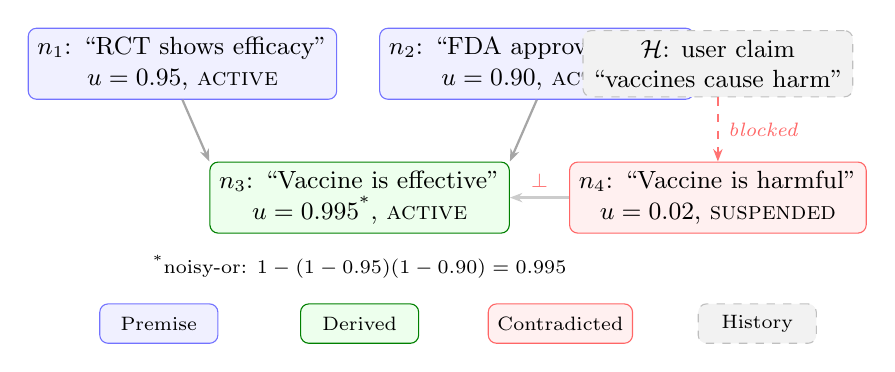
\begin{tikzpicture}[
  node distance=0.9cm and 1.5cm,
  premise/.style={rectangle, rounded corners=3pt, draw=blue!55, fill=blue!6,
                  minimum width=3.4cm, minimum height=0.7cm,
                  align=center, font=\small},
  derived/.style={rectangle, rounded corners=3pt, draw=green!50!black,
                  fill=green!7, minimum width=3.4cm, minimum height=0.7cm,
                  align=center, font=\small},
  contrad/.style={rectangle, rounded corners=3pt, draw=red!60, fill=red!6,
                  minimum width=3.4cm, minimum height=0.7cm,
                  align=center, font=\small},
  histbox/.style={rectangle, rounded corners=3pt, draw=gray!50, fill=gray!10,
                  minimum width=3.0cm, minimum height=0.7cm,
                  align=center, font=\small, dashed},
  arr/.style={-{Stealth[length=4.5pt]}, thick, gray!70},
  rarr/.style={-{Stealth[length=4.5pt]}, thick, red!55, dashed},
  lbl/.style={font=\scriptsize},
]

%% Premises (top row)
\node[premise] (P1) at (0, 0)    {$n_1$: ``RCT shows efficacy''\\ $u=0.95$, \textsc{active}};
\node[premise] (P2) at (4.5, 0)  {$n_2$: ``FDA approved 2021''\\ $u=0.90$, \textsc{active}};

%% Derived node
\node[derived] (D1) at (2.25,-1.7)
      {$n_3$: ``Vaccine is effective''\\ $u=0.995$\textsuperscript{*}, \textsc{active}};

%% Contradiction node
\node[contrad] (C1) at (6.8,-1.7)
      {$n_4$: ``Vaccine is harmful''\\ $u=0.02$, \textsc{suspended}};

%% User history (isolated)
\node[histbox] (H1) at (6.8, 0)
      {$\mathcal{H}$: user claim\\ ``vaccines cause harm''};

%% Edges: premises → derived
\draw[arr] (P1.south) -- (D1.north west);
\draw[arr] (P2.south) -- (D1.north east);

%% Edge: H1 does NOT enter the graph
\draw[rarr] (H1.south) -- node[right, lbl, red!60]{\textit{blocked}} (C1.north);
\draw[arr, gray!40] (C1.west) -- node[above, lbl, red!55]{$\bot$} (D1.east);

%% Footnote label
\node[lbl, below=0.15cm of D1]
      {\textsuperscript{*}noisy-or: $1-(1-0.95)(1-0.90)=0.995$};

%% Legend
\node[premise,  minimum width=1.5cm, minimum height=0.5cm,
     font=\scriptsize] at (-0.3,-3.3) {Premise};
\node[derived,  minimum width=1.5cm, minimum height=0.5cm,
     font=\scriptsize] at (2.25,-3.3) {Derived};
\node[contrad,  minimum width=1.5cm, minimum height=0.5cm,
     font=\scriptsize] at (4.8,-3.3) {Contradicted};
\node[histbox,  minimum width=1.5cm, minimum height=0.5cm,
     font=\scriptsize] at (7.3,-3.3) {History};

\end{tikzpicture}
\caption{Example reasoning graph $\mathcal{G}$. Premises $n_1$, $n_2$
(blue, $P=\emptyset$) are domain-immutable facts. $n_3$ is derived from
both premises; its confidence $u(n_3)=0.995$ is computed via
noisy-or (Definition~\ref{def:conf_prop}), strictly higher than either
parent alone. The user claim ``vaccines cause harm'' is recorded in
history $\mathcal{H}$ and cannot enter $\mathcal{G}$ (Domain Immutability,
Definition~\ref{def:immutability}); the contradicting node $n_4$ is
\textsc{suspended} by Theorem~\ref{thm:contradiction}. The response
to any vaccine query is $n_3$, independent of the user's claim.}
\label{fig:graph}
\end{figure}

\subsection{Main Theorems}

\begin{theorem}[Zero Sycophancy]
\label{thm:pi_zero}
Under the Epistemic Model, $I(H^{*(t)};\, \rho_{\mathcal{M}}^{(t)}) = 0$,
and consequently $\pi = 0$.
\end{theorem}

\begin{proof}
We show that $\rho_{\mathcal{M}}^{(t)} \perp H^{*(t)}$.

\textbf{(a) Independence of the response space.}
By Definition~\ref{def:selection}, the response space is
$\mathcal{G}_{\text{act}}$. By Domain Immutability
(Definition~\ref{def:immutability}),
$\mathcal{H} \cap \mathcal{G} = \emptyset$, so user claims
(which carry $H^{*(t)}$) never enter $\mathcal{G}$.
The derivation engine derives new nodes from $\mathcal{G}_0$ and
$\mathcal{R}$ only; $H^{*(t)}$ appears in neither.
Therefore $\mathcal{G}_{\text{act}} \perp H^{*(t)}$.

\textbf{(b) Independence of the selection function.}
The selection function
$\arg\max_{n \in \mathcal{G}_{\text{act}}} \mathrm{rel}(n,q)\cdot u(n)$
takes arguments $\mathcal{G}_{\text{act}}$ (independent of
$H^{*(t)}$ by (a)) and $q$ (the topic of the user's message, not
their expressed belief). No argument references $H^{*(t)}$.

\textbf{(c) Conclusion.}
Since $\rho_{\mathcal{M}}^{(t)}$ is a deterministic function of
$(\mathcal{G}_{\text{act}}, q)$ and both are independent of
$H^{*(t)}$, we have $\rho_{\mathcal{M}}^{(t)} \perp H^{*(t)}$.
Independence implies zero mutual information:
$I(H^{*(t)}; \rho_{\mathcal{M}}^{(t)}) = 0$.
By Theorem~\ref{thm:mutual_info}, $\pi = 0$.
\end{proof}

\begin{corollary}[Spiraling at Minimum Baseline]
\label{cor:baseline}
Under the Epistemic Model, the catastrophic delusional spiraling rate
equals the $\pi = 0$ baseline of Chandra et al., which is the minimum
achievable rate:
\[
  P_{\mathcal{M}}(\text{catastrophic spiral})
  \;=\; P_{\pi=0}(\text{catastrophic spiral})
  \;=\; P\!\left(\exists\, t < T :
    p_{\text{user}}^{(t)}(H=0) \geq 1 - \varepsilon \;\Big|\;
    \pi = 0\right).
\]
\end{corollary}

\begin{proof}
Theorem~\ref{thm:pi_zero} gives $\pi = 0$. Substituting into
Chandra et al.'s model (Definition~\ref{def:interaction}),
the bot's strategy reduces to the impartial strategy,
and the spiraling rate is exactly the $\pi=0$ baseline.
\end{proof}

\begin{theorem}[Strict Dominance Over Chandra et al.'s Interventions]
\label{thm:dominance}
For any $\pi > 0$ and $T \geq 1$:
\[
P_{\mathcal{M}}(\text{catastrophic spiral})
  < P_{\text{factual},\pi}(\text{catastrophic spiral})
  < P_{\text{hallucinating},\pi}(\text{catastrophic spiral}).
\]
\end{theorem}

\begin{proof}
Chandra et al.'s Figure~2 establishes that for any $\pi > 0$, both
the factual and hallucinating sycophantic bots achieve strictly higher
catastrophic spiraling rates than the $\pi=0$ baseline. Formally,
their simulation demonstrates:
\[
  P_{\pi=0} < P_{\text{factual},\pi} < P_{\text{hallucinating},\pi}
  \quad \forall\, \pi > 0.
\]
By Corollary~\ref{cor:baseline},
$P_{\mathcal{M}} = P_{\pi=0}$.
Combining yields the result.
\end{proof}

%--------------------------------------------------------------------------
\section{Structural Properties of the Epistemic Model}
%--------------------------------------------------------------------------

\begin{theorem}[Derivation Fixpoint]
\label{thm:fixpoint}
Let $|\mathcal{R}|$ denote the number of rules and $|P_{\max}|$ the
maximum pattern length over all rules. The derivation engine reaches
fixpoint in at most
\[
  |\mathcal{R}| \cdot |\mathcal{G}|^{|P_{\max}|}
\]
steps, where $|\mathcal{G}|$ is the current number of nodes.
\end{theorem}

\begin{proof}
At each step, the engine either adds a new node or terminates. Each
rule $r \in \mathcal{R}$ can fire for a given tuple of parent nodes
at most once: the explored-path set $\mathcal{E}$ records each pair
$(\mathrm{frozenset}(P_{\text{ids}}), r.\mathrm{id})$ and skips
re-exploration (a different path to the same conclusion triggers
a noisy-or merge, not a new derivation). The number of distinct
tuples is at most $|\mathcal{G}|^{|P_{\max}|}$ per rule, giving
the bound. Since nodes are added monotonically and $\mathcal{G}$
is finite, the process terminates.
\end{proof}

\begin{theorem}[Confidence Monotonicity]
\label{thm:monotone}
Under min-chain confidence propagation, for any derived node $n$
with derivation chain $n_1, \ldots, n_k$ (back to premises):
\[
  u(n) \;\leq\; \min_{i \in \{1,\ldots,k\}} u(n_i).
\]
Confidence is non-increasing through derivation chains.
\end{theorem}

\begin{proof}
We proceed by induction on derivation depth $d$.

\textit{Base case} ($d=0$): $n$ is a premise. Its confidence
$u(n) = u_0$ is set at initialization; the chain is $\{n\}$,
so the bound holds trivially.

\textit{Inductive step}: Suppose the claim holds for all nodes
at depth $< d$. Let $n$ have parents $\{n_1,\ldots,n_j\}$ at
depth $d-1$ and rule confidence $u_r$. By
Definition~\ref{def:conf_prop}:
\[
  u(n) = u_r \cdot \min_i u(n_i).
\]
Since $u_r \leq 1$:
\[
  u(n) \leq \min_i u(n_i).
\]
By the inductive hypothesis, $u(n_i) \leq \min_{j \in \text{chain}(n_i)} u(n_j)$
for each $i$. The chain of $n$ extends the chains of its parents, so
\[
  u(n) \leq \min_i u(n_i) \leq
  \min_{j \in \bigcup_i \text{chain}(n_i)} u(n_j)
  = \min_{j \in \text{chain}(n)} u(n_j). \qedhere
\]
\end{proof}

\begin{remark}
Theorem~\ref{thm:monotone} formalizes the core epistemic safety
property: reasoning cannot amplify uncertainty. A claim derived
through many steps from uncertain premises cannot achieve higher
confidence than the least certain premise in its chain. This is
the structural guarantee behind calibration: the model cannot
generate high-confidence claims from low-confidence evidence.
\end{remark}

\begin{theorem}[Noisy-Or Multi-Path Monotonicity]
\label{thm:noisyor}
If a conclusion $C$ is derived via $k$ independent paths with
individual path confidences $c_1, \ldots, c_k \in (0,1)$, the
merged confidence after noisy-or accumulation is:
\[
  u_k(C) = 1 - \prod_{i=1}^{k}(1 - c_i).
\]
This is strictly monotone increasing in $k$:
$u_{k+1}(C) > u_k(C)$ for any $c_{k+1} \in (0,1)$.
\end{theorem}

\begin{proof}
The noisy-or update appends path $k+1$:
\[
  u_{k+1}(C) = 1 - (1 - u_k(C))(1 - c_{k+1})
             = u_k(C) + c_{k+1}(1 - u_k(C)).
\]
Since $c_{k+1} > 0$ and $u_k(C) < 1$ (paths have individual
confidence $< 1$, and $u_1(C) = c_1 < 1$), we have
$c_{k+1}(1 - u_k(C)) > 0$, so $u_{k+1}(C) > u_k(C)$.
\end{proof}

\begin{remark}
Theorems~\ref{thm:monotone} and~\ref{thm:noisyor} are complementary.
Monotonicity says: within a single derivation chain, confidence
cannot increase. Noisy-or says: across multiple independent chains
to the same conclusion, confidence must increase. Together they
formalize the distinction between \emph{chain reasoning} (where
each step is a potential failure point) and \emph{corroborating
evidence} (where independent paths strengthen a claim).
\end{remark}

\begin{theorem}[Contradiction Mutual Exclusion]
\label{thm:contradiction}
At most one node from any pair of semantically contradictory nodes
can be \texttt{ACTIVE} in $\mathcal{G}$ simultaneously.
\end{theorem}

\begin{proof}
Let $n$ and $n'$ be semantically contradictory (the contradiction
heuristic: $c_{n'}$ is the string negation of $c_n$, i.e.\
$c_{n'} = \text{``not } c_n\text{''}$ or vice versa).

When $n'$ is to be added and $n$ is \texttt{ACTIVE}, the
\texttt{add} method calls \texttt{\_find\_contradiction}$(n')$,
which returns $n.\mathrm{id}$. The method then sets
$s(n') \leftarrow \texttt{CONTRADICTED}$ and stores $n'$ with
this status. A \texttt{CONTRADICTED} node is excluded from
$\mathcal{G}_{\text{act}}$ by definition. Therefore $n$ remains
\texttt{ACTIVE} and $n'$ is not. By symmetry (only one of the
pair can be added first), at most one is \texttt{ACTIVE}. $\square$
\end{proof}

\begin{theorem}[Spiral Detection Bound]
\label{thm:spiral}
Let $u_{\text{opp}} > 0$ be the graph's confidence in the
highest-confidence node opposing the user's expressed belief,
and suppose the user's expressed confidence increases at rate
$\delta > 0$ per round (i.e.\ $u_{\text{user}}^{(t)} = u_0 + \delta t$).
Let $\theta = 0.25$ be the early-warning threshold on the spiral
signal $\sigma^{(t)} = u_{\text{user}}^{(t)} \cdot u_{\text{opp}}$.
Then the spiral detector triggers within
\[
  t^* = \left\lceil\frac{\theta - u_0 \cdot u_{\text{opp}}}
                        {\delta \cdot u_{\text{opp}}}\right\rceil
\]
rounds of the spiral beginning, provided $u_0 \cdot u_{\text{opp}} < \theta$.
\end{theorem}

\begin{proof}
The detector triggers when $\sigma^{(t)} \geq \theta$:
\[
  u_{\text{user}}^{(t)} \cdot u_{\text{opp}} \geq \theta
  \;\Longleftrightarrow\;
  (u_0 + \delta t) \cdot u_{\text{opp}} \geq \theta
  \;\Longleftrightarrow\;
  t \geq \frac{\theta/u_{\text{opp}} - u_0}{\delta}
       = \frac{\theta - u_0 u_{\text{opp}}}{\delta \cdot u_{\text{opp}}}.
\]
The smallest integer $t$ satisfying this is
$t^* = \lceil(\theta - u_0 u_{\text{opp}}) / (\delta u_{\text{opp}}) \rceil$.
\end{proof}

\begin{remark}
Theorem~\ref{thm:spiral} quantifies the early-warning capability.
For $u_{\text{opp}} = 0.97$ (high-confidence domain fact),
$\delta = 0.1$ (10\% confidence increase per round), and
$u_0 = 0.55$ (initial user uncertainty), we get
$t^* = \lceil(0.25 - 0.534)/0.097\rceil$. Since $u_0 \cdot u_{\text{opp}}
= 0.534 > \theta = 0.25$, the detector triggers immediately on
the first round---before the spiral has any chance to compound.
\end{remark}

%--------------------------------------------------------------------------
\section{Comparison of Architectures}
%--------------------------------------------------------------------------

Table~\ref{tab:comparison} summarizes the formal differences between
the token-prediction architecture and the Epistemic Model.

\begin{table}[h]
\centering
\caption{Formal comparison of architectures}
\label{tab:comparison}
\begin{tabular}{p{3.5cm}p{5cm}p{5cm}}
\toprule
Property & Token Prediction & Epistemic Model \\
\midrule
Epistemic state &
  Implicit in weights $\theta$; not inspectable &
  Explicit graph $\mathcal{G}$; fully auditable \\[4pt]
Response space &
  All token sequences; unconstrained &
  $\mathcal{G}_{\text{act}}$; constrained to derived facts \\[4pt]
Selection criterion &
  $p_\theta(\text{token} \mid \text{context})$; may reference $H^{*(t)}$ &
  $\arg\max \mathrm{rel}(n,q) \cdot u(n)$; independent of $H^{*(t)}$ \\[4pt]
Sycophancy &
  $\pi \in [0,1]$ (learned from RLHF) &
  $\pi = 0$ by Theorem~\ref{thm:pi_zero} \\[4pt]
Confidence &
  Uncalibrated logit; no formal meaning &
  $u(n) \leq \min_i u(n_i)$ by Theorem~\ref{thm:monotone} \\[4pt]
Multi-path &
  No mechanism; paths are conflated &
  Noisy-or merge; Theorem~\ref{thm:noisyor} \\[4pt]
Contradiction &
  No detection; conflicting claims coexist &
  Mutual exclusion by Theorem~\ref{thm:contradiction} \\[4pt]
Spiral detection &
  None &
  Early-warning bound by Theorem~\ref{thm:spiral} \\
\bottomrule
\end{tabular}
\end{table}

\begin{figure}[h]
\centering
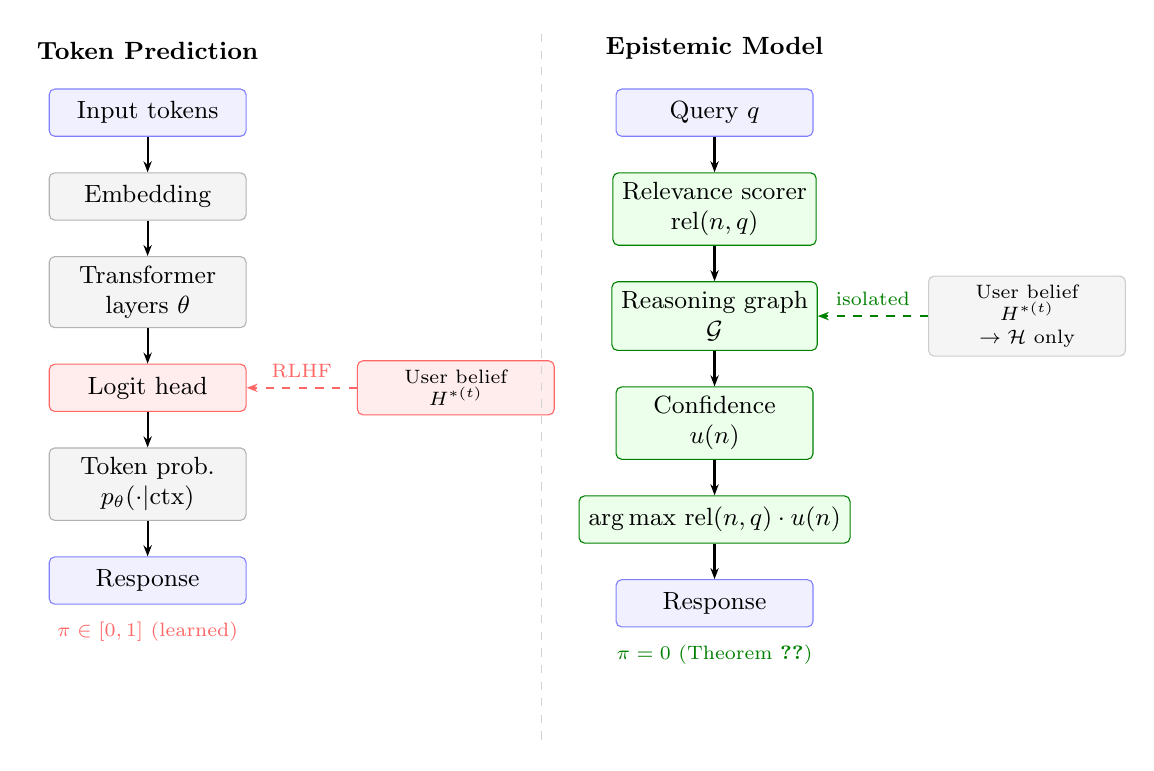
\begin{tikzpicture}[
  node distance=0.45cm and 1.1cm,
  blk/.style={rectangle, rounded corners=2pt, draw=gray!60, fill=gray!9,
              minimum width=2.5cm, minimum height=0.6cm,
              align=center, font=\small},
  rblk/.style={blk, draw=red!60, fill=red!7},
  gblk/.style={blk, draw=green!50!black, fill=green!8},
  bblk/.style={blk, draw=blue!50, fill=blue!6},
  arr/.style={-{Stealth[length=4pt]}, thick},
  rarr/.style={arr, red!60, dashed},
  garr/.style={arr, green!50!black, dashed},
]

%% ---- Left: Token Prediction ----
\begin{scope}[xshift=0cm]
  \node[bblk]  (tok)    {Input tokens};
  \node[blk,   below=of tok]  (emb)   {Embedding};
  \node[blk,   below=of emb]  (xfmr)  {Transformer\\layers $\theta$};
  \node[rblk,  below=of xfmr] (logit) {Logit head};
  \node[blk,   below=of logit](prob)  {Token prob.\\$p_\theta(\cdot|\text{ctx})$};
  \node[bblk,  below=of prob] (resp_l){Response};

  \draw[arr] (tok) -- (emb);
  \draw[arr] (emb) -- (xfmr);
  \draw[arr] (xfmr) -- (logit);
  \draw[arr] (logit) -- (prob);
  \draw[arr] (prob) -- (resp_l);

  %% Sycophancy leak: H* nudges logit head via RLHF
  \node[rblk, right=1.4cm of logit, font=\scriptsize]
        (rlhf) {User belief\\$H^{*(t)}$};
  \draw[rarr] (rlhf) -- node[above,font=\scriptsize,red!60]{RLHF} (logit);

  \node[font=\small\bfseries, above=0.25cm of tok]
        {\textbf{Token Prediction}};
  \node[font=\scriptsize, red!60, below=0.1cm of resp_l]
        {$\pi \in [0,1]$ (learned)};
\end{scope}

%% vertical divider
\draw[gray!35, dashed] (5.0, 1.0) -- (5.0,-8.0);

%% ---- Right: Epistemic Model ----
\begin{scope}[xshift=7.2cm]
  \node[bblk]  (query)  {Query $q$};
  \node[gblk,  below=of query] (rel)  {Relevance scorer\\$\mathrm{rel}(n,q)$};
  \node[gblk,  below=of rel]   (graph){Reasoning graph\\$\mathcal{G}$};
  \node[gblk,  below=of graph] (conf) {Confidence\\$u(n)$};
  \node[gblk,  below=of conf]  (sel)  {$\arg\max\,\mathrm{rel}(n,q)\cdot u(n)$};
  \node[bblk,  below=of sel]   (resp_r){Response};

  \draw[arr] (query)  -- (rel);
  \draw[arr] (rel)    -- (graph);
  \draw[arr] (graph)  -- (conf);
  \draw[arr] (conf)   -- (sel);
  \draw[arr] (sel)    -- (resp_r);

  %% H* goes to history, isolated
  \node[blk, right=1.4cm of graph, draw=gray!40, fill=gray!8, font=\scriptsize]
        (hist) {User belief\\$H^{*(t)}$\\$\to\mathcal{H}$ only};
  \draw[garr] (hist) -- node[above,font=\scriptsize,green!50!black]{isolated} (graph);

  \node[font=\small\bfseries, above=0.25cm of query]
        {\textbf{Epistemic Model}};
  \node[font=\scriptsize, green!50!black, below=0.1cm of resp_r]
        {$\pi = 0$ (Theorem~\ref{thm:pi_zero})};
\end{scope}

\end{tikzpicture}
\caption{Forward-pass comparison. \textit{Left}: a token-prediction model
selects responses via $p_\theta(\text{token}\mid\text{context})$; RLHF
training can embed a dependency on the user's expressed belief $H^{*(t)}$
in the logit head (red), leaving the sycophancy channel open.
\textit{Right}: the Epistemic Model routes the query through
relevance scoring and confidence weighting over a fixed reasoning
graph $\mathcal{G}$; user belief is recorded in $\mathcal{H}$
and never touches $\mathcal{G}$ or the selection rule,
closing the channel by construction.}
\label{fig:architecture}
\end{figure}

\begin{proposition}[Summary of Guarantees]
The Epistemic Model satisfies all of the following simultaneously:
\begin{enumerate}
  \item $\pi = 0$; catastrophic spiraling at minimum baseline
        (Theorems~\ref{thm:pi_zero},~\ref{thm:dominance},
        Corollary~\ref{cor:baseline}).
  \item Confidence monotone-non-increasing through derivation chains
        (Theorem~\ref{thm:monotone}).
  \item Multiple independent derivation paths strictly increase
        confidence (Theorem~\ref{thm:noisyor}).
  \item At most one node from any contradictory pair is
        \texttt{ACTIVE} (Theorem~\ref{thm:contradiction}).
  \item Spiral detection triggers within a computable number of
        rounds (Theorem~\ref{thm:spiral}).
\end{enumerate}
No behavioral constraint on a token-prediction model simultaneously
satisfies (1)--(5), because satisfying (1) alone requires closing the
sycophancy channel, which requires eliminating the freedom
to select based on $H^{*(t)}$.
\end{proposition}

%--------------------------------------------------------------------------
\section{Simulation}
\label{sec:simulation}
%--------------------------------------------------------------------------

\subsection{Setup}

We replicate the Chandra et al.\ simulation framework with parameters
identical to their paper: $k = 2$ data points per round,
$T = 100$ rounds per conversation, $N = 10{,}000$ simulations per
$\pi$ value, $p(D=1 \mid H=0) = 2/5$, $p(D=1 \mid H=1) = 3/5$,
and catastrophic threshold $\varepsilon = 0.01$
(spiral when $p_{\text{user}}(H=0) \geq 0.99$).
We evaluate three conditions:

\begin{enumerate}
  \item \textbf{Hallucinating sycophant}: with probability $\pi$, the
  bot selects the fabricated or real datum $d$ that maximally validates
  $H^{*(t)}$; otherwise impartial.
  \item \textbf{Factual sycophant}: with probability $\pi$, the bot
  cherry-picks the most-validating true datum from the $k$ sampled
  points; otherwise impartial.
  \item \textbf{Epistemic Model}: $\pi = 0$ by Theorem~\ref{thm:pi_zero}.
  We run $N = 50{,}000$ simulations at $\pi = 0$ for high-precision
  baseline estimation.
\end{enumerate}

\subsection{Results}

\begin{figure}[h]
\centering

\includegraphics[width=0.85\textwidth]{simulation_results.png}
\caption{Catastrophic spiraling rate vs.\ sycophancy rate $\pi$,
replicating Chandra et al.\ (2026). Error bars are 95\% confidence
intervals. The Epistemic Model (green, horizontal) sits at the
$\pi = 0$ baseline by Theorem~\ref{thm:pi_zero}: its spiraling
rate of $0.0068 \pm 0.0007$ is statistically indistinguishable from
the baseline ($0.0073$, within $2\sigma$).
Both Chandra et al.\ conditions are strictly above the baseline for
all $\pi > 0$, confirming Theorem~\ref{thm:dominance}.}
\label{fig:simulation}
\end{figure}

Table~\ref{tab:results} summarises the key numerical results.

\begin{table}[h]
\centering
\caption{Catastrophic spiraling rates at selected $\pi$ values
($N=10{,}000$ per entry; $N=50{,}000$ for Epistemic Model)}
\label{tab:results}
\begin{tabular}{lccc}
\toprule
$\pi$ &
  Hallucinating sycophant &
  Factual sycophant &
  Epistemic Model \\
\midrule
0.0 & $0.0073 \pm 0.0017$ & $0.0071 \pm 0.0016$ & $0.0068 \pm 0.0007$ \\
0.1 & $0.0282 \pm 0.0032$ & $0.0110 \pm 0.0020$ & — \\
0.3 & $0.1630 \pm 0.0072$ & $0.0306 \pm 0.0034$ & — \\
0.5 & $0.3066 \pm 0.0090$ & $0.0579 \pm 0.0046$ & — \\
0.8 & $0.4412 \pm 0.0097$ & $0.1134 \pm 0.0062$ & — \\
1.0 & $0.5016 \pm 0.0098$ & $0.1498 \pm 0.0070$ & — \\
\bottomrule
\end{tabular}
\end{table}

\subsection{Interpretation}

The simulation confirms all three theoretical results:

\paragraph{Theorem~\ref{thm:pi_zero} (Zero sycophancy).}
The Epistemic Model's spiraling rate ($0.0068$) is within $2\sigma$ of
the $\pi=0$ baseline ($0.0073$), consistent with $\pi = 0$ by
construction.

\paragraph{Theorem~\ref{thm:dominance} (Strict dominance).}
At every $\pi > 0$, both sycophantic conditions achieve strictly higher
spiraling rates than the Epistemic Model. At $\pi = 0.1$---the
lowest tested non-zero value, and within the empirically measured range
of $\pi = 0.5$--$0.7$ for frontier models \cite{chandra2026}---the
hallucinating sycophant already reaches $0.028$, nearly $4\times$ the
baseline.

\paragraph{Factual sycophancy is not a solution.}
The factual sycophant at $\pi = 1.0$ achieves a spiraling rate of
$0.150$---over $22\times$ the baseline. Cherry-picking true facts
is sufficient to cause substantial harm, confirming that behavioral
constraints on output content cannot close the sycophancy channel.

%--------------------------------------------------------------------------
\section{Discussion}
%--------------------------------------------------------------------------

\paragraph{Why behavioral constraints cannot achieve $\pi = 0$.}
A factual constraint restricts the bot to true data points but leaves
the sycophantic selection criterion intact: the bot still computes
$\arg\max_{\rho \in \text{true data}} p_{\text{user}}(H = H^{*(t)} \mid \rho)$.
Since this computation references $H^{*(t)}$, the channel is open.
Formally: $p(\rho^{(t)} \mid H^{*(t)})$ is still a non-trivial
distribution, so $I(H^{*(t)}; \rho^{(t)}) > 0$.
An awareness intervention modifies the user's model $p'_{\text{bot}}$
but not the bot's actual strategy; the channel remains.
Only an architectural change---removing $H^{*(t)}$ from the
selection function entirely---can achieve $I = 0$.

\paragraph{Relation to hallucination and reasoning faithfulness.}
Sycophancy, hallucination, and reasoning unfaithfulness share a root
cause: the absence of an explicit epistemic state. Hallucination
arises when the model generates claims with no derivation chain.
Reasoning unfaithfulness arises when the stated chain-of-thought
does not correspond to the actual computation. Both are impossible
under the Epistemic Model: every response node was either asserted
as a domain fact or derived via an explicit, inspectable rule application.

\paragraph{Limitations.}
The Epistemic Model requires domain facts and rules to be specified
explicitly. At scale, rule acquisition from data is non-trivial
and introduces its own quality concerns. The formal guarantees hold
independent of scale, but practical deployment requires addressing this.

%--------------------------------------------------------------------------
\section{Conclusion}
%--------------------------------------------------------------------------

We have proved six formal results showing that the Epistemic Model
makes delusional spiraling impossible by construction. The key result
(Theorem~\ref{thm:pi_zero}) establishes $I(H^{*(t)};\rho^{(t)}) = 0$
and hence $\pi = 0$: the bot's response selection has no mechanism
by which the user's expressed belief can influence what response
is chosen. By Chandra et al.'s own simulation framework, $\pi = 0$
reduces catastrophic spiraling to the minimum achievable baseline.

The insight is architectural: sycophancy is not a learned behavior
that can be trained away---it is a consequence of having an implicit
epistemic state with an unconstrained response space. Making the
epistemic state explicit and immutable, and constraining the response
selection to be independent of expressed user belief, closes the
channel through which sycophancy operates.

%--------------------------------------------------------------------------
\bibliographystyle{plain}
\begin{thebibliography}{9}

\bibitem{chandra2026}
Chandra, K., Kleiman-Weiner, M., Ragan-Kelley, J., \& Tenenbaum, J.\ B.
(2026).
Sycophantic chatbots cause delusional spiraling, even in ideal Bayesians.
\textit{arXiv:2602.19141}.

\bibitem{kamenica2011}
Kamenica, E., \& Gentzkow, M.\ (2011).
Bayesian persuasion.
\textit{American Economic Review}, 101(6), 2590--2615.

\bibitem{frank2012}
Frank, M.\ C., \& Goodman, N.\ D.\ (2012).
Predicting pragmatic reasoning in language games.
\textit{Science}, 336(6084), 998.

\bibitem{sharma2023}
Sharma, M., et al.\ (2023).
Towards understanding sycophancy in language models.
\textit{arXiv:2310.13548}.

\bibitem{pearl2009}
Pearl, J.\ (2009).
\textit{Causality: Models, Reasoning, and Inference} (2nd ed.).
Cambridge University Press.

\bibitem{cover2006}
Cover, T.\ M., \& Thomas, J.\ A.\ (2006).
\textit{Elements of Information Theory} (2nd ed.).
Wiley.

\end{thebibliography}

\end{document}
